% 第 11 题图乙：磁传感器记录的 B-t 图像（pgfplots 重绘）
% 0~t0 内有 10 个完整波形，故 T = t0/10
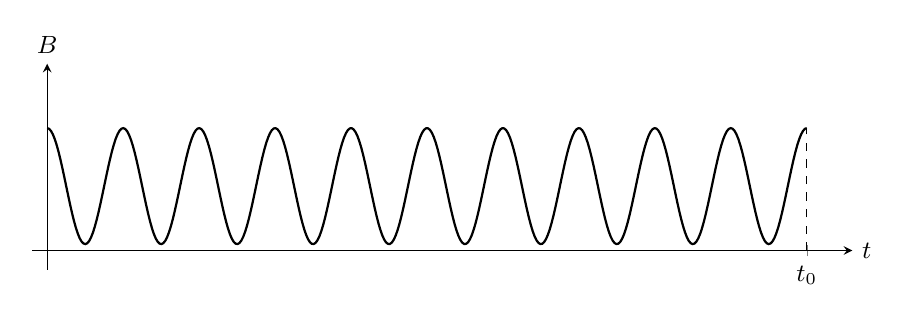
\begin{tikzpicture}
  \begin{axis}[
      width=12cm, height=4.2cm,
      axis lines=middle,
      xlabel={$t$}, ylabel={$B$},
      xmin=-0.2, xmax=10.6, ymin=-0.15, ymax=1.45,
      xtick={10}, xticklabels={$t_0$},
      ytick=\empty,
      xlabel style={anchor=west}, ylabel style={anchor=south},
      font=\small, clip=false]
    \addplot[thick, domain=0:10, samples=400] {0.5+0.45*cos(deg(2*pi*x))};
    \draw[dashed] (axis cs:10,0) -- (axis cs:10,0.95);
  \end{axis}
\end{tikzpicture}
